\section{Light Capturing Devices}
This section deals with the basic evolution of light capturing devices.
\subsection{Notes}
Initially, there was a single cell 1D capture of light. This had many problems, but the main one being it can only capture light from one direction, and had no understanding of the intensity of it (binary). Using multiple 1D Cells allowed for more directions to be captured.
\begin{figure}[!htb]
	\center{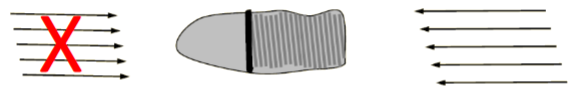
\includegraphics[width=10cm]
		{vision/1dcell}}
	\caption{\label{fig:1dcell} 1D Cell}
\end{figure}
Having multiple cells curved allowed for capture of light from various directions, somewhat conic. But it had difficulty keeping track of an image, as the same image would be hitting too many cells, so it would be all over the place.
\begin{figure}[!htb]
	\center{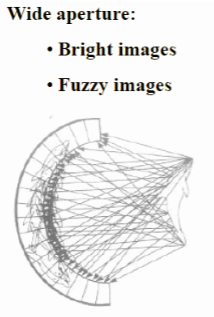
\includegraphics[width=4cm]
		{vision/wideaperture}}
	\caption{\label{fig:1dlinearcell} 1D Cell Curved Array}
\end{figure}
The concept of a pinhole camera was the next step, but there was an issue. With the wide aperture, the images were bright but they were fuzzy. With the pinhole, the images were sharp but they were too dim. How can we get the positives without the negatives?
\begin{figure}[!htb]
	\center{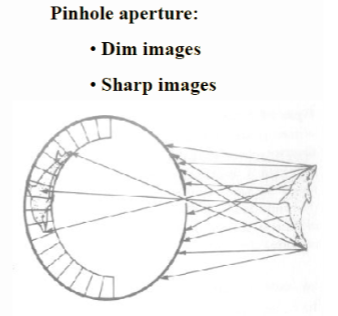
\includegraphics[width=4cm]
		{vision/pinholeaperture}}
	\caption{\label{fig:pinholeaperture} Pinhole}
\end{figure}
Simple, refraction from lenses. By having a lens refract light into the pinhole camera, or image point, it would allow for all the light to pass through the pinhole and hit different cells based on the initial angle the light hit the lens, maintaining the brightness from the wide aperture with the clarity of the pinhole aperture.

The virtual image created is upside down, and our eyes, based on this concept, simply allow the brain to flip it back.
\begin{figure}[!htb]
	\center{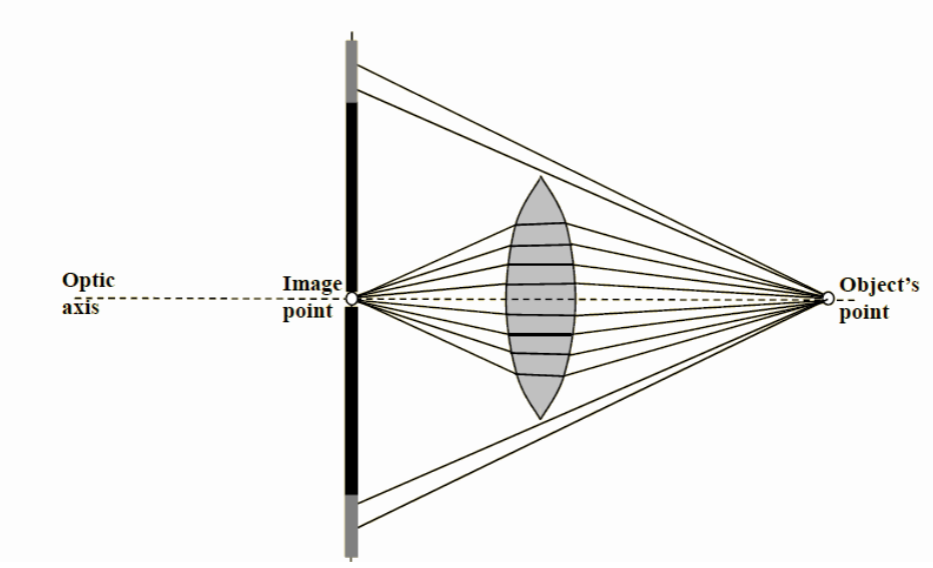
\includegraphics[width=5cm]
		{vision/lens}}
	\caption{\label{fig:lens} Lens in action}
\end{figure}
\section{Human Vision}
This section deals with human vision, a fairly straight forward topic.
\subsection{Notes}
The human retina contains two types of photo receptor cells. Rods, of where there are ~120 million, and Cones, of which there are ~6 million. Rods are exetremely sensitive to light and respond to single photons. They have poor spatial resolutions as multiple of them converge to the same neuron for data handling. However, thanks to their sensitivity, they help us see light in the dark.
This is different with cones, which are active at higher light levels. Several neurons process Cone data, so they have higher spatial resolution than rods.

\textbf{Receptive Field}

The receptive field is the area on which light must fall for neurons to be stimulated.The size of a receptive field determines a few things. Small receptive fields are stimulated by high spatial frequencies; and large spatial fields are stimulated by low spatial frequencies.  There are differences between the centre and periphery of field. We can't talk about these without talking about ganglion cells.
\begin{figure}[!htb]
	\center{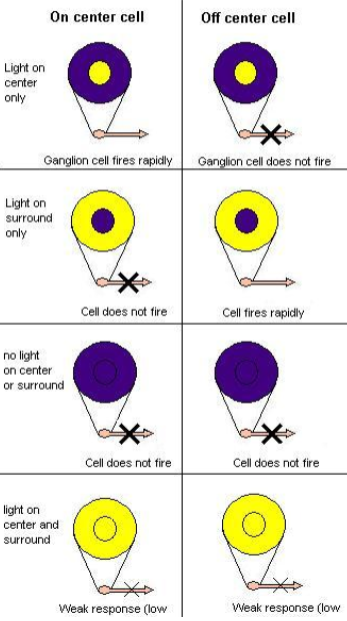
\includegraphics[width=6cm]
		{vision/ganglion}}
	\caption{\label{fig:lens} Ganglion responses}
\end{figure}
There are two types of ganglion cells, on-center and off-center, as seen in the image. On-center cells are stimulated when the center is exposed to light, and are inhibited when the surrounded area is exposed. This works opposite for off-center cells, as the name suggests.

Ganglion cells have a higher action potential rate depending on the intensity and location of light hit. This allows us to have a grasp at contrast, as it responds differently to different intensities of light.

\textbf{Visual Pathway}

\begin{enumerate}
	\item Vision generated by photoreceptors in the eyes (as explained above)
	\item The information leaves the eye by way of the optic nerve. Special note: The humans have a blind spot in the eye that does not allow them to see at one specific part of the eye; this is the optic nerve's location. Without it, we wouldn't be able to actually see.
	\item There is a partial crossing of axons at the optic chiasm; this allows the brain to receive data on the same visual field from both eyes, superimposing images, creating a sense of depth, etc.
	\item The axos following the chiasm, also known as the optic tract, wraps around the midbrain to get to the lateral geniculate nucleus (LGN).
	\item The LGN axons fan out to the deep white matter of the brain before ultimately traveling to the primary visual cortex at the back of the brain, where the magic happens.
\end{enumerate}
\begin{figure}[!htb]
	\center{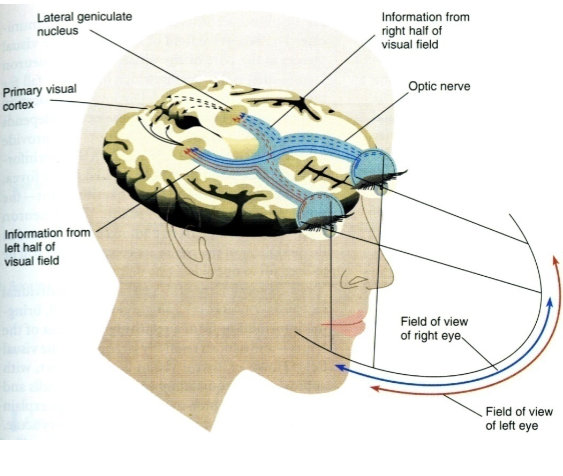
\includegraphics[width=5cm]
		{vision/visualpathway}}
	\caption{\label{fig:lens} Visualising the visual pathway}
\end{figure}
